\documentclass[12pt,a4paper]{article}


\usepackage[margin=1in]{geometry}
\usepackage{amsmath,amssymb,bm,mathtools}
\usepackage{siunitx}
\usepackage{graphicx}
\usepackage{booktabs}
\usepackage{array}
\usepackage{float}
\usepackage{xcolor}
\usepackage{caption}
\usepackage{subcaption}
\usepackage{listings}
\usepackage{tikz}
\usepackage{pgfplots}
\usepackage[hidelinks]{hyperref}
\usepackage{enumitem}
\usepackage{placeins}
\usepackage{pdflscape}
\pgfplotsset{compat=1.18}
\usepackage{wrapfig}
\usepackage{rotating}


\lstdefinestyle{cleanPython}{
    language=Python,
    basicstyle=\ttfamily\small,
    keywordstyle=\bfseries,
    stringstyle=\itshape,
    numbers=left,
    numberstyle=\tiny,
    stepnumber=1,
    numbersep=8pt,
    frame=single,
    breaklines=true,
    showstringspaces=false,
    tabsize=4,
    captionpos=b
}

\lstdefinestyle{cleanText}{
    basicstyle=\ttfamily\small,
    numbers=left,
    numberstyle=\tiny,
    stepnumber=1,
    numbersep=8pt,
    frame=single,
    breaklines=true,
    showstringspaces=false,
    tabsize=4,
    captionpos=b
}



\begin{document}
\begin{titlepage}
    \centering
    \vspace*{0.7cm}
    \includegraphics[width=0.62\textwidth]{Picture1.png}
    
    \vspace{1.5cm}
    {\Huge \textbf{Numerical Modeling of Ground Effect and Downforce in Formula 1 Vehicles}\par}

    \vspace{0.7cm}

   
    {\Large \textbf{Course}\par}

    \vspace{0.5cm}

    {\large MTH 221 -- Math 4 (Spring 2026)\par}

    \vspace{0.7cm}

    {\Large \textbf{Course Report}\par}

    \vspace{0.5cm}

    {\large Numerical Modeling / CFD\par}
    {\large Probability and Statistics\par}
    \vspace{0.5cm}

 \vspace{0.5cm}

{\Large \textbf{Team Members}\par}

\vspace{0.4cm}

\begin{flushleft}
\large

\textbf{1.} \textbf{Name:} Felopater Edwar \hfill \textbf{ID:} 120240336

\vspace{0.2cm}

\textbf{2.} \textbf{Name:} \dotfill \hfill \textbf{ID:} \dotfill

\vspace{0.2cm}

\textbf{3.} \textbf{Name:} \dotfill \hfill \textbf{ID:} \dotfill

\vspace{0.2cm}

\textbf{4.} \textbf{Name:} \dotfill \hfill \textbf{ID:} \dotfill

\vspace{0.2cm}

\textbf{5.} \textbf{Name:} \dotfill \hfill \textbf{ID:} \dotfill

\vspace{0.2cm}

\textbf{6.} \textbf{Name:} \dotfill \hfill \textbf{ID:} \dotfill

\vspace{0.2cm}

\textbf{7.} \textbf{Name:} \dotfill \hfill \textbf{ID:} \dotfill

\vspace{0.2cm}

\textbf{8.} \textbf{Name:}\dotfill \hfill \textbf{ID:} \dotfill

\vspace{0.2cm}

\textbf{9.} \textbf{Name:} \dotfill \hfill \textbf{ID:} \dotfill

\vspace{0.2cm}

\textbf{10.} \textbf{Name:} \dotfill \hfill \textbf{ID:} \dotfill

\end{flushleft}

\vfill
\end{titlepage}


\newpage
\tableofcontents
\newpage

\section{Introduction}

\subsection{Background Information}

The dynamic behavior of a Formula 1 car is largely determined by its aerodynamic
performance, particularly at high speeds, where aerodynamic forces become more dominant
than purely mechanical forces. Among these aerodynamic forces, downforce plays one of
the most important roles because it increases tire grip, improves cornering ability, and
enhances braking efficiency. Unlike drag, which negatively affects the straight-line speed
of the vehicle, downforce provides a net performance advantage by allowing the car to
maintain higher speeds through corners without compromising stability.

\vspace{10pt}

Ground effect is the primary mechanism for generating downforce

\begin{wrapfigure}{r}{0.42\textwidth}
    \centering
    \vspace{-12pt}
    \includegraphics[width=\linewidth]{Picture1.jpg}
    \caption{The underbody model for F1 cars in 2022 compared to 2021.}
    \label{fig:underbody_comparison}
    \vspace{-10pt}
\end{wrapfigure}

in modern Formula 1
cars. It results from the interaction between the airflow under the vehicle and the ground
surface. The underbody geometry is optimized to accelerate the airflow through the
constricted region between the car floor and the track. As the airflow speed increases
under the car, the static pressure decreases. This pressure reduction creates a pressure
difference between the lower and upper surfaces of the vehicle, generating a downward
force that pulls the car toward the ground.

\vspace{10pt}

The magnitude of this effect is strongly affected by geometric parameters such as ride
height, floor curvature, underfloor shape, and diffuser expansion angle. Therefore, ground
effect is considered a highly sensitive and nonlinear aerodynamic phenomenon. For this
reason, it can be clearly observed in newer Formula 1 cars compared with older designs,
as modern cars are designed to generate a stronger suction region under the floor, as
shown in Figure 1.

\vspace{10pt}

The reintroduction of ground-effect-based regulations in contemporary Formula 1 design
has shifted the main source of downforce from external aerodynamic elements, such as
front and rear wings, toward the underbody of the car. This transition aims to improve
aerodynamic efficiency by producing higher downforce-to-drag ratios while reducing the
sensitivity of the wake flow behind the car. As a result, closer racing conditions can be
achieved because the following car experiences less disturbed airflow. However, the
performance of ground effect systems is strongly influenced by flow separation, vortex
formation, and boundary layer behavior, especially under varying operating conditions.

\vspace{10pt}

Analytical methods alone are usually not sufficient to predict the aerodynamic behavior
of a Formula 1 vehicle because the flow around the car involves complex geometry,
turbulence, separation, pressure recovery, and wake formation. Computational Fluid
Dynamics (CFD) enables the numerical solution of the governing fluid-flow equations
over complex geometries. It also allows the analysis of detailed velocity fields, pressure
distributions, streamline patterns, and the mechanisms responsible for lift, drag, and
downforce production.

\vspace{10pt}

The use of suitable discretization techniques and turbulence models helps in understanding
the behavior of turbulent boundary layers, flow separation, and wake structures, all of
which directly affect ground-effect performance. Therefore, in order to identify optimal
design solutions, the effect of each design parameter on aerodynamic performance must
be investigated sequentially and under controlled numerical conditions.

\vspace{10pt}

This report presents a numerical analysis of the ground effect and its contribution to
downforce generation in a Formula 1 vehicle. The investigation involves modeling the
airflow around a simplified vehicle geometry and examining the effect of key variables,
such as ride height and underbody configuration, on the aerodynamic performance of
the vehicle. The numerical method used in this study is based on CFD techniques for
solving the governing equations of fluid motion.

\subsection{Mathematical Formulation}

The aerodynamic behavior of the vehicle is governed by the fundamental conservation
laws of fluid mechanics. These laws describe how mass, momentum, pressure, and velocity
interact within the flow field. In this study, the most important governing relations are
the continuity equation, the Navier--Stokes equations, Reynolds number, Bernoulli's
principle, downforce equation, and drag force equation.

\subsubsection{Law of Conservation of Mass: Continuity Equation}

The law of conservation of mass states that mass cannot be created or destroyed. For
fluid flow, this means that the mass flow rate entering a control volume must be equal
to the mass flow rate leaving it, provided that there is no accumulation of mass inside
the control volume.

For incompressible flow, the continuity equation can be written as:

\begin{equation}
    \nabla \cdot \vec{V} = 0
    \label{eq:continuity_vector}
\end{equation}

where $\vec{V}$ is the velocity vector of the flow.

For a simple one-dimensional passage, the continuity principle can also be expressed as:

\begin{equation}
    \rho A V = \text{constant}
    \label{eq:continuity_1d}
\end{equation}

where $\rho$ is the fluid density, $A$ is the cross-sectional area, and $V$ is the flow
velocity.

This equation helps explain the Venturi effect. When the airflow is forced through a
smaller passage under the Formula 1 car, the flow area decreases. According to the
continuity equation, the velocity must increase. This increase in velocity is one of the
main reasons for the pressure reduction under the car floor.

\subsubsection{Law of Conservation of Momentum: Navier--Stokes Equations}

The law of conservation of momentum describes how the velocity of air changes due to
the forces acting on the fluid. These forces include pressure forces and viscous friction
forces. The incompressible Navier--Stokes equation can be expressed as:

\begin{equation}
    \rho \left(
    \frac{\partial \vec{V}}{\partial t}
    +
    (\vec{V} \cdot \nabla)\vec{V}
    \right)
    =
    -\nabla P
    +
    \mu \nabla^2 \vec{V}
    \label{eq:navier_stokes}
\end{equation}

where $\rho$ is the air density, $\vec{V}$ is the velocity vector, $P$ is the static pressure,
and $\mu$ is the dynamic viscosity.

The left-hand side of Equation~\ref{eq:navier_stokes} represents the momentum change
of the fluid. The right-hand side represents the forces acting on the fluid. The term
$\frac{\partial \vec{V}}{\partial t}$ is the local acceleration, which describes the change
of velocity with time. The term $(\vec{V} \cdot \nabla)\vec{V}$ is the convective acceleration,
which represents the momentum change caused by the fluid moving through regions of
different velocity. The term $-\nabla P$ is the pressure-gradient force, which drives the
air from high-pressure regions to low-pressure regions. Finally, the term
$\mu \nabla^2 \vec{V}$ represents viscous friction, which slows the airflow near solid
surfaces such as the car body, floor, and diffuser walls.

For turbulent aerodynamic flow, the Reynolds-Averaged Navier--Stokes equations are
commonly used instead of solving all turbulent fluctuations directly. This allows the
mean flow field to be solved while the effect of turbulence is represented using a
turbulence model.

\subsubsection{Reynolds Number}

Before solving any aerodynamic problem, the nature of the airflow must be identified.
The flow may be laminar, transitional, or turbulent. Reynolds number expresses the ratio
between inertial forces and viscous forces and is used to determine the dominant flow
behavior.

The Reynolds number is given by:

\begin{equation}
    Re = \frac{\rho V L}{\mu} = \frac{V L}{\nu} \label{eq:reynolds}
\end{equation}

where $\rho$ is the fluid density, $V$ is the characteristic velocity, $L$ is the characteristic
length, $\mu$ is the dynamic viscosity, and $\nu$ is the kinematic viscosity.

In Formula 1 applications, the Reynolds number is usually very high because the vehicle
moves at high speed and has a relatively large characteristic length. Therefore, the flow
around the car is generally turbulent. This justifies the use of turbulence modeling in
the CFD simulation.

\subsubsection{Bernoulli's Principle and Ground Effect}

The core physical principle behind ground-effect downforce is related to Bernoulli's
equation. As the car floor gets closer to the ground, the air is forced through a narrowing
channel. Due to the continuity equation, the air velocity increases in this restricted
region. According to Bernoulli's principle, an increase in flow velocity is associated with
a reduction in static pressure.

Bernoulli's equation can be written as:

\begin{equation}
    P + \frac{1}{2}\rho V^2 + \rho g h = \text{constant}
    \label{eq:bernoulli}
\end{equation}

where $P$ is the static pressure, $\frac{1}{2}\rho V^2$ is the dynamic pressure, and
$\rho g h$ is the potential energy per unit volume due to elevation.

In the underfloor region of a Formula 1 car, the height variation is usually small compared
with the effect of velocity change. Therefore, the main relationship can be simplified
conceptually as: when velocity increases, static pressure decreases. This pressure drop
under the car creates suction and contributes directly to downforce generation.

\subsubsection{Downforce}

Downforce is the net aerodynamic force that pushes the vehicle downward toward the
track. In coefficient form, the aerodynamic lift force is calculated as:

\begin{equation}
    L = \frac{1}{2}\rho V^2 A C_L
    \label{eq:lift_coefficient}
\end{equation}

where $\rho$ is the air density, $V$ is the vehicle speed, $A$ is the reference area, and
$C_L$ is the lift coefficient.

For a Formula 1 car, the desired lift is negative. Therefore, the downforce can be written as:

\begin{equation}
    F_{\text{downforce}} = -L
    \label{eq:downforce}
\end{equation}

A more precise expression for the aerodynamic force is obtained by integrating pressure
and viscous shear stress over the surface of the vehicle:

\begin{equation}
    \vec{F} = \int_A \left(-P \vec{n}  + \vec{\tau}  \right) \, dA
    \label{eq:surface_force}
\end{equation}

where $\vec{n}$ is the surface normal vector, $\vec{\tau}$ is the shear stress vector, and
$dA$ is an infinitesimal surface area.

The vertical component of Equation~\ref{eq:surface_force} gives the lift force. If this
vertical force acts downward, it is considered downforce. The main reason for downforce
generation in the ground-effect region is the low-pressure zone formed under the car floor
and diffuser.

\subsubsection{Drag Force}

Drag force is the aerodynamic resistance acting opposite to the direction of vehicle
motion. It reduces the straight-line speed of the car and increases the power required
from the engine. The drag force can be calculated using:

\begin{equation}
    D = \frac{1}{2}\rho V^2 A C_D
    \label{eq:drag_force}
\end{equation}

where $\rho$ is the air density, $A$ is the reference area, $V$ is the vehicle speed, and
$C_D$ is the drag coefficient.

For a more precise calculation, the same surface-force integral in
Equation~\ref{eq:surface_force} can be used, but the force is resolved in the horizontal
direction instead of the vertical direction.

The aerodynamic design objective is not only to maximize downforce, but also to keep
drag within an acceptable range. Therefore, the aerodynamic efficiency can be evaluated
using the downforce-to-drag ratio:

\begin{equation}
    \eta = \frac{F_{\text{downforce}}}{D}
    \label{eq:aero_efficiency}
\end{equation}

A higher value of $\eta$ indicates that the car produces a large amount of downforce for
a relatively small amount of drag, which is desirable in Formula 1 aerodynamic design.

\subsection{Applied Numerical Example: Downforce Estimation for a Realistic Formula 1 Case}

To connect the mathematical formulation with a practical engineering case, a simplified
numerical example is considered. Assume that a Formula 1 car is moving at a speed of
$V = 50~\text{m/s}$ with air density $\rho = 1.225~\text{kg/m}^3$ and reference area
$A = 1.5~\text{m}^2$. For a selected ride height of $40~\text{mm}$, the CFD simulation
predicts a lift coefficient of:

\begin{equation}
    C_L = -2.35
\end{equation}

The dynamic pressure is calculated from:

\begin{equation}
    q = \frac{1}{2}\rho V^2
\end{equation}

Substituting the values:

\begin{equation}
    q = \frac{1}{2}(1.225)(50)^2
\end{equation}

\begin{equation}
    q = 1531.25~\text{Pa}
\end{equation}

The aerodynamic lift force is:

\begin{equation}
    L = C_L q A
\end{equation}

\begin{equation}
    L = (-2.35)(1531.25)(1.5)
\end{equation}

\begin{equation}
    L = -5397.2~\text{N}
\end{equation}

Since Formula 1 cars require negative lift, the downforce is:

\begin{equation}
    F_{\text{downforce}} = -L
\end{equation}

\begin{equation}
    F_{\text{downforce}} = 5397.2~\text{N}
\end{equation}

This means that at a ride height of $40~\text{mm}$ and a vehicle speed of $50~\text{m/s}$,
the aerodynamic system generates approximately:

\begin{equation}
    F_{\text{downforce}} \approx 5.4~\text{kN}
\end{equation}

This downward force increases the normal load on the tires, improving cornering grip
without increasing the actual mass of the car.

If the drag coefficient for the same case is:

\begin{equation}
    C_D = 0.88
\end{equation}

then the drag force is:

\begin{equation}
    D = C_D q A
\end{equation}

\begin{equation}
    D = (0.88)(1531.25)(1.5)
\end{equation}

\begin{equation}
    D = 2021.3~\text{N}
\end{equation}

The aerodynamic efficiency is therefore:

\begin{equation}
    \eta = \frac{F_{\text{downforce}}}{D}
\end{equation}

\begin{equation}
    \eta = \frac{5397.2}{2021.3}
\end{equation}

\begin{equation}
    \eta = 2.67
\end{equation}

Therefore, for every $1~\text{N}$ of drag produced, the car generates approximately
$2.67~\text{N}$ of downforce. This indicates that the selected ride height gives strong
ground-effect performance and represents an efficient aerodynamic operating condition.

This example shows that the equations are not only theoretical; they can be used directly
to estimate the aerodynamic performance of a real vehicle configuration. The negative
value of $C_L$ confirms that the force acts downward, while the high downforce-to-drag
ratio shows that the underfloor and diffuser are working efficiently.

\clearpage
\begin{landscape}
\begin{figure}[p]
    \centering
    \includegraphics[width=0.98\linewidth,height=0.78\textheight,keepaspectratio]{ChatGPT Image May 7, 2026, 06_20_11 PM}
    \caption{High-detail engineering visualization of the applied numerical example for a simplified Formula 1 vehicle. The figure combines the analytical force estimation with a 3D representation of the vehicle geometry, computational domain, ride height, and static pressure contours responsible for downforce generation.}
    \label{fig:applied_example_f1}
\end{figure}
\end{landscape}
\clearpage

\FloatBarrier


\section{Discretization and Numerical Strategy}

\subsection{Finite Volume Method}

The Finite Volume Method is used to discretize the governing equations. The computational domain is divided into small control volumes. The conservation equations are integrated over each control volume.

The general steady transport equation is:

\begin{equation}
    \nabla \cdot (\rho \bm{u}\phi)
    =
    \nabla \cdot (\Gamma \nabla \phi) + S_{\phi}
\end{equation}

After integration over a control volume \(V_P\):

\begin{equation}
    \int_{V_P} \nabla \cdot (\rho \bm{u}\phi)\,dV
    =
    \int_{V_P} \nabla \cdot (\Gamma \nabla \phi)\,dV
    +
    \int_{V_P} S_{\phi}\,dV
\end{equation}

Using Gauss' divergence theorem:

\begin{equation}
    \sum_f\left(\rho \bm{u}_f \cdot \bm{n}_f \right) \phi_f A_f = \sum_f \Gamma_f \left( \nabla \phi \right)_f\cdot \bm{n}_f A_f + S_{\phi}V_P
\end{equation}

where \(f\) represents the faces of the control volume.

\subsection{Discretized Algebraic Equation}

For each cell \(P\), the discretized equation can be written as:

\begin{equation}
    a_P \phi_P = \sum_{nb} a_{nb}\phi_{nb} + b_P
\end{equation}

where:
\begin{itemize}
    \item \(a_P\) is the central coefficient,
    \item \(a_{nb}\) are neighbor-cell coefficients,
    \item \(\phi_P\) is the value at the current cell,
    \item \(\phi_{nb}\) are neighboring values,
    \item \(b_P\) is the source term.
\end{itemize}

For a 2D structured mesh, this equation becomes:

\begin{equation}
    a_P\phi_P = a_E\phi_E + a_W\phi_W + a_N\phi_N + a_S\phi_S + b_P
\end{equation}

where \(E,W,N,S\) represent east, west, north, and south neighboring cells.

\subsection{Coefficient Matrix Form}

For the entire computational domain, all cell equations are assembled into a matrix system:

\begin{equation}
    \bm{A}\bm{\Phi} = \bm{b}
\end{equation}

where:

\begin{equation}
\bm{A}
=
\begin{bmatrix}
a_{P1} & -a_{12} & 0 & \cdots & 0 \\
-a_{21} & a_{P2} & -a_{23} & \cdots & 0 \\
0 & -a_{32} & a_{P3} & \cdots & 0 \\
\vdots & \vdots & \vdots & \ddots & -a_{n-1,n} \\
0 & 0 & 0 & -a_{n,n-1} & a_{Pn}
\end{bmatrix}
\end{equation}

\begin{equation}
\bm{\Phi}
=
\begin{bmatrix}
\phi_1\\
\phi_2\\
\phi_3\\
\vdots\\
\phi_n
\end{bmatrix},
\qquad
\bm{b}
=
\begin{bmatrix}
b_1\\
b_2\\
b_3\\
\vdots\\
b_n
\end{bmatrix}
\end{equation}

This matrix is sparse because each cell is only connected to its neighboring cells. In a real CFD solver, separate matrix systems are solved for:

\begin{itemize}
    \item \(u\)-momentum,
    \item \(v\)-momentum,
    \item \(w\)-momentum,
    \item pressure correction,
    \item turbulence variable \(k\),
    \item turbulence variable \(\omega\).
\end{itemize}

\subsection{Momentum Equation Matrix}

For the \(u\)-velocity component, the discretized equation is:

\begin{equation}
    a_P^u u_P =\sum_{nb} a_{nb}^u u_{nb}+b_P^u-\left(\frac{\partial p}{\partial x} \right)_P V_P
\end{equation}

Similarly, for the \(v\)-velocity component:

\begin{equation}
    a_P^v v_P = \sum_{nb} a_{nb}^v v_{nb} + b_P^v - \left(  \frac{\partial p}{\partial y}    \right)_P V_P
\end{equation}

In matrix form:

\begin{equation}
    \bm{A}_u\bm{u} = \bm{b}_u - \bm{G}_x\bm{p}
\end{equation}

\begin{equation}
    \bm{A}_v\bm{v} = \bm{b}_v - \bm{G}_y\bm{p}
\end{equation}

where \(\bm{G}_x\) and \(\bm{G}_y\) are pressure gradient operators.

\subsection{Pressure Correction Equation}

In incompressible flow, the velocity field must satisfy:

\begin{equation}
    \nabla \cdot \bm{u} = 0
\end{equation}

The SIMPLE algorithm introduces pressure and velocity corrections:

\begin{equation}
    p = p^* + p'
\end{equation}

\begin{equation}
    u = u^* + u'
\end{equation}

\begin{equation}
    v = v^* + v'
\end{equation}

The velocity correction is related to pressure correction:

\begin{equation}
    u' = -d_u \frac{\partial p'}{\partial x}
\end{equation}

\begin{equation}
    v' = -d_v \frac{\partial p'}{\partial y}
\end{equation}

Substituting these corrections into the continuity equation gives the pressure correction equation:

\begin{equation}
    a_P^{p'} p'_P = a_E^{p'} p'_E + a_W^{p'} p'_W + a_N^{p'} p'_N + a_S^{p'} p'_S + b_P^{p'}
\end{equation}

In matrix form:

\begin{equation}
    \bm{A}_{p'}\bm{p}' = \bm{b}_{p'}
\end{equation}

This pressure correction equation is the numerical core of incompressible CFD because it forces the velocity field to satisfy mass conservation.

\subsection{Turbulence Model Equations}

The selected turbulence model is \(k-\omega\) SST. In simplified form, it solves two transport equations.

\subsubsection{Turbulent Kinetic Energy Equation}

\begin{equation}
    \frac{\partial (\rho k)}{\partial t} + \nabla \cdot (\rho \bm{u} k) = \nabla\cdot \left[ \left( \mu + \sigma_k \mu_t  \right) \nabla k \right] +P_k  - \beta^* \rho k \omega
\end{equation}

\subsubsection{Specific Dissipation Rate Equation}

\begin{equation}
    \frac{\partial (\rho \omega)}{\partial t}+ \nabla \cdot (\rho \bm{u} \omega) = \nabla \cdot \left[ \left(\mu + \sigma_{\omega} \mu_t\right)\nabla \omega\right]+\alpha \frac{\omega}{k}P_k -\beta \rho \omega^2
\end{equation}

The turbulent viscosity is calculated as:

\begin{equation}
    \mu_t = \rho \frac{k}{\omega}
\end{equation}

In the SST formulation, blending functions are used to improve behavior near walls and in free-stream regions.

\subsection{Numerical Schemes Used}

The following numerical schemes are used:

\begin{table}[H]
\centering
\caption{Numerical schemes used in the simulation}
\begin{tabular}{llp{6cm}}
\toprule
\textbf{Term} & \textbf{Scheme} & \textbf{Reason} \\
\midrule
Gradient & Least Squares Cell-Based & Accurate for unstructured CFD meshes \\
Pressure & Second Order & Better pressure prediction under the car \\
Momentum & Second-Order Upwind & Captures velocity gradients more accurately \\
Turbulent kinetic energy \(k\) & Second-Order Upwind & Reduces numerical diffusion \\
Specific dissipation rate \(\omega\) & Second-Order Upwind & Better near-wall turbulence prediction \\
Pressure-velocity coupling & SIMPLE & Suitable for steady incompressible flow \\
\bottomrule
\end{tabular}
\end{table}

\subsection{Under-Relaxation Factors}

Under-relaxation is used to stabilize the iterative solution. Instead of applying the full new value directly, only part of it is accepted.

\begin{equation}
    \phi^{new} = \phi^{old} + \alpha \left( \phi^{calculated} - \phi^{old} \right)
\end{equation}

where \(\alpha\) is the under-relaxation factor.

Typical values are:

\begin{table}[H]
\centering
\caption{Suggested under-relaxation factors}
\begin{tabular}{lc}
\toprule
\textbf{Variable} & \textbf{Under-relaxation factor} \\
\midrule
Pressure & 0.3 \\
Momentum & 0.7 \\
Turbulent kinetic energy \(k\) & 0.8 \\
Specific dissipation rate \(\omega\) & 0.8 \\
Turbulent viscosity & 1.0 \\
\bottomrule
\end{tabular}
\end{table}

\subsection{Linear Solvers}

Each discretized equation produces a sparse linear system:

\begin{equation}
    \bm{A}\bm{x} = \bm{b}
\end{equation}

For pressure correction, an iterative solver such as Algebraic Multigrid is commonly used. For momentum and turbulence equations, Gauss-Seidel or conjugate-gradient-type solvers may be used depending on the CFD software.

The reason iterative solvers are preferred is that the number of cells can be very large, often millions of cells, so direct matrix inversion is computationally expensive.


\section{Algorithm Implementation and Code}

\subsection{Numerical Algorithm}

The numerical algorithm used in this study follows the SIMPLE procedure:

\begin{enumerate}
    \item Initialize pressure, velocity, turbulence variables, and material properties.
    \item Solve the discretized momentum equations using the guessed pressure field.
    \item Obtain tentative velocities \(u^*,v^*,w^*\).
    \item Assemble the pressure correction matrix.
    \item Solve the pressure correction equation.
    \item Correct pressure.
    \item Correct velocity components.
    \item Solve turbulence equations for \(k\) and \(\omega\).
    \item Update turbulent viscosity.
    \item Recalculate fluxes through cell faces.
    \item Check residuals and force coefficients.
    \item Repeat until convergence.
\end{enumerate}

\subsection{Pseudocode of the Numerical Solver}

\begin{lstlisting}[style=cleanText, caption={Detailed SIMPLE-based CFD algorithm}]
Start

Read geometry and mesh

Initialize:
    velocity field U
    pressure field p
    turbulent kinetic energy k
    specific dissipation rate omega
    turbulent viscosity mu_t

Set boundary conditions:
    velocity inlet
    pressure outlet
    no-slip car body
    moving ground
    slip or symmetry side boundaries

For each iteration:

    1. Assemble momentum matrices:
        A_u * u = b_u - G_x * p
        A_v * v = b_v - G_y * p
        A_w * w = b_w - G_z * p

    2. Solve momentum equations:
        u_star = solve(A_u, rhs_u)
        v_star = solve(A_v, rhs_v)
        w_star = solve(A_w, rhs_w)

    3. Compute mass fluxes at cell faces

    4. Assemble pressure correction matrix:
        A_pprime * p_prime = b_pprime

    5. Solve pressure correction equation:
        p_prime = solve(A_pprime, b_pprime)

    6. Correct pressure:
        p_new = p_old + alpha_p * p_prime

    7. Correct velocity:
        u_new = u_star + u_correction
        v_new = v_star + v_correction
        w_new = w_star + w_correction

    8. Solve turbulence equations:
        A_k * k = b_k
        A_omega * omega = b_omega

    9. Update turbulent viscosity:
        mu_t = rho * k / omega

    10. Apply under-relaxation

    11. Calculate residuals

    12. Calculate aerodynamic forces:
        lift
        drag
        downforce

    13. Check convergence:
        residuals < 1e-5
        downforce is stable
        drag is stable

End loop

Post-process:
    pressure contours
    velocity contours
    streamlines
    downforce vs ride height
    downforce vs diffuser angle
    grid convergence

End
\end{lstlisting}


\subsection{Numerical Solver Implementation Framework}

The implementation presented in this section is divided into two levels. The first level
describes the CFD solver framework required to solve the governing equations using the
Finite Volume Method, the SIMPLE pressure--velocity coupling algorithm, and the
$k-\omega$ SST turbulence model. The second level presents a simplified Python
post-processing code used to calculate aerodynamic forces and compare numerical cases
using representative aerodynamic coefficients.

This distinction is important because a full industrial CFD solver requires complex
geometry handling, mesh generation, turbulence wall treatment, and iterative sparse
linear-system solution. Therefore, the solver framework described here represents the
numerical logic and algorithmic structure required for the Formula 1 ground-effect
problem, while the Python code that follows is used to organize the numerical results,
calculate forces, and generate plots.

\subsubsection{Implementation Overview}

The simplified solver is assumed to be implemented in Python using scientific computing
libraries. NumPy is used for numerical arrays, SciPy sparse solvers are used for solving
linear systems, and Matplotlib is used for post-processing and plotting. The physical
domain is modeled using a two-dimensional structured Cartesian mesh in order to simplify
the underfloor flow problem while still capturing the main ground-effect behavior.

The main numerical features of the implementation are:

\begin{itemize}
    \item finite volume discretization of the governing equations,
    \item structured two-dimensional computational grid,
    \item SIMPLE pressure--velocity coupling,
    \item sparse matrix solution for momentum and pressure correction,
    \item $k-\omega$ SST turbulence closure,
    \item boundary-condition enforcement at inlet, outlet, wall, ground, and symmetry boundaries,
    \item aerodynamic force calculation from pressure and wall shear stress,
    \item parametric comparison of ride height and diffuser angle effects.
\end{itemize}

\subsubsection{Code Module Structure}

The numerical implementation can be organized into self-contained modules. Each module
corresponds to a physical or numerical part of the CFD formulation.

\begin{table}[H]
\centering
\caption{Suggested code module structure for the Formula 1 ground-effect solver.}
\label{tab:code_module_structure}
\begin{tabular}{p{6cm}p{10.5cm}}
\toprule
\textbf{Module / Function} & \textbf{Responsibility} \\
\midrule
\text{Sim Parameters} & Stores physical constants and solver settings such as air density, viscosity, inlet velocity, grid size, ride height, and under-relaxation factors. \\
\text{Grid} & Generates the computational mesh and maps two-dimensional cell indices into one-dimensional matrix indices. \\
\text{Flow Field} & Stores flow variables such as $u$, $v$, $p$, $k$, $\omega$, and turbulent viscosity $\mu_t$. \\
\text{compute turbulent viscosity} & Computes turbulent viscosity using the simplified relation $\mu_t = \rho k/\omega$. \\
\text{compute face coefficients} & Calculates convection--diffusion coefficients at cell faces. \\
\text{solve momentum} & Assembles and solves the discretized $u$- and $v$-momentum equations. \\
\texttt{pressure correction} & Assembles and solves the SIMPLE pressure-correction equation. \\
\text{solve turbulence} & Solves the transport equations for $k$ and $\omega$. \\
\text{apply boundary conditions} & Applies inlet, outlet, car wall, moving ground, and symmetry boundary conditions. \\
\text{compute aerodynamic forces} & Calculates downforce and drag from pressure and shear-stress integration. \\
\texttt{run simple} & Controls the main SIMPLE iteration loop until convergence. \\
\texttt{post process} & Generates pressure contours, velocity plots, streamlines, and result tables. \\
\texttt{ride height study} & Runs a parametric sweep to study the effect of ride height on downforce. \\
\bottomrule
\end{tabular}
\end{table}

\subsubsection{Simulation Parameters}

All physical and numerical parameters are stored in one location to make the code easier
to modify and extend. The main parameters used in the simplified implementation are
shown in Table~\ref{tab:simulation_parameters}.

\begin{table}[H]
\centering
\caption{Main simulation parameters used in the simplified solver framework.}
\label{tab:simulation_parameters}
\begin{tabular}{p{3cm}p{5.5cm}p{3cm}p{2cm}}
\toprule
\textbf{Variable} & \textbf{Description} & \textbf{Value / Formula} & \textbf{Unit} \\
\midrule
$\rho$ & Air density & 1.225 & kg/m$^3$ \\
$\mu$ & Dynamic viscosity & $1.81\times10^{-5}$ & Pa$\cdot$s \\
$V_{\infty}$ & Free-stream velocity & 50.0 & m/s \\
$L_{\text{ref}}$ & Reference length & 1.0 & m \\
$Re$ & Reynolds number & $\rho V_{\infty}L_{\text{ref}}/\mu$ & -- \\
$N_x \times N_y$ & Grid resolution & $120 \times 40$ & cells \\
$h$ & Ride height & 0.04--0.05 & m \\
$\alpha_u$ & Momentum under-relaxation & 0.7 & -- \\
$\alpha_p$ & Pressure under-relaxation & 0.3 & -- \\
\bottomrule
\end{tabular}
\end{table}

A simplified Python-style representation of these parameters is:

\begin{lstlisting}[style=cleanPython, caption={Simulation parameters for the simplified CFD framework.}]
class SimParameters:
    rho = 1.225          # kg/m^3 air density
    mu = 1.81e-5         # Pa.s dynamic viscosity
    V_inf = 50.0         # m/s free-stream velocity
    L_ref = 1.0          # m reference length
    Nx, Ny = 120, 40     # grid resolution
    ride_height = 0.04   # m ground clearance
    alpha_u = 0.7        # momentum under-relaxation
    alpha_p = 0.3        # pressure under-relaxation
\end{lstlisting}

\subsubsection{Grid Generation}

A structured Cartesian grid is used to divide the two-dimensional computational domain
into finite volumes. Cell centers are placed at the midpoint of each control volume. The
underbody region is identified by comparing the vertical coordinate of each cell with the
specified ride height. This allows the code to isolate the ground-effect region where
pressure reduction and suction are expected to occur.

\begin{lstlisting}[style=cleanPython, caption={Simplified grid generation and cell-index mapping.}]
class Grid:
    def __init__(self, p):
        self.Nx = p.Nx
        self.Ny = p.Ny

        self.Lx = 6.0
        self.Ly = 2.0

        self.dx = self.Lx / self.Nx
        self.dy = self.Ly / self.Ny

        self.x = np.linspace(self.dx/2, self.Lx - self.dx/2, self.Nx)
        self.y = np.linspace(self.dy/2, self.Ly - self.dy/2, self.Ny)

        self.X, self.Y = np.meshgrid(self.x, self.y, indexing="ij")

        # Cells inside the underbody / ground-effect region
        self.underbody_mask = self.Y <= p.ride_height

    def cell_index(self, i, j):
        return i * self.Ny + j
\end{lstlisting}

\subsubsection{SIMPLE Iteration Loop}

The Semi-Implicit Method for Pressure-Linked Equations, known as SIMPLE, is used to
couple pressure and velocity in incompressible flow. The algorithm starts with an initial
guess for pressure and velocity, solves the momentum equations, corrects pressure and
velocity using a pressure-correction equation, and repeats the process until convergence.

The simplified SIMPLE loop can be written as:

\begin{lstlisting}[style=cleanText, caption={SIMPLE outer iteration loop for the simplified CFD solver.}]
Initialize:
    u = V_inf
    v = 0
    p = 0
    k = k_initial
    omega = omega_initial

For each iteration:

    1. Compute turbulent viscosity:
        mu_t = rho * k / omega

    2. Assemble convection-diffusion coefficients.

    3. Solve momentum prediction equations:
        A_u * u_star = b_u - G_x * p
        A_v * v_star = b_v - G_y * p

    4. Compute face mass fluxes.

    5. Assemble pressure-correction equation:
        A_pprime * p_prime = b_pprime

    6. Correct pressure:
        p_new = p_old + alpha_p * p_prime

    7. Correct velocity:
        u_new = u_star + u_correction
        v_new = v_star + v_correction

    8. Solve turbulence equations for k and omega.

    9. Apply boundary conditions.

    10. Compute residuals and aerodynamic coefficients.

    11. Stop if:
        residual < tolerance
        C_L and C_D become stable
\end{lstlisting}

\subsubsection{Momentum Equation Solver}

Following the discretized momentum equation, the velocity components are solved using
a sparse linear system. For the $x$-momentum equation, the general form is:

\begin{equation}
    A_u u^* = b_u - G_x p
\end{equation}

where $u^*$ is the predicted velocity, $A_u$ is the momentum coefficient matrix, $b_u$
is the source vector, and $G_xp$ represents the pressure-gradient contribution.

During the assembly process, under-relaxation is applied to improve numerical stability:

\begin{equation}
    \frac{a_P}{\alpha_u}u_P^* = \sum_{nb}a_{nb}u_{nb}^* +b_P+\frac{1-\alpha_u}{\alpha_u}a_P u_P^{old}
\end{equation}

A simplified Python-style structure is shown below:

\begin{lstlisting}[style=cleanPython, caption={Simplified momentum-equation solver structure.}]
def solve_momentum(grid, field, p):
    aE, aW, aN, aS, aP = compute_face_coefficients(grid, field, p)

    N = grid.Nx * grid.Ny
    A = lil_matrix((N, N))
    rhs = np.zeros(N)

    for i in range(grid.Nx):
        for j in range(grid.Ny):
            idx = grid.cell_index(i, j)

            A[idx, idx] = aP[i, j] / p.alpha_u

            # Neighbor coefficients are inserted if the neighbors exist
            # A[idx, east]  = -aE[i, j]
            # A[idx, west]  = -aW[i, j]
            # A[idx, north] = -aN[i, j]
            # A[idx, south] = -aS[i, j]

            rhs[idx] = source[i, j] + \
                (1 - p.alpha_u) / p.alpha_u * aP[i, j] * field.u[i, j]

    u_star = spsolve(csr_matrix(A), rhs).reshape(grid.Nx, grid.Ny)

    return u_star
\end{lstlisting}






\subsubsection{Pressure-Correction Equation}

After solving the momentum equations, the predicted velocity field does not necessarily
satisfy continuity. Therefore, the pressure-correction equation is assembled from the
local mass-flux imbalance.

The pressure correction equation has the form:

\begin{equation}
    A_{p'}p' = b_{p'}
\end{equation}

where $p'$ is the pressure correction and $b_{p'}$ is related to the mass imbalance at
the control-volume faces. The velocity and pressure fields are corrected as:

\begin{equation}
    p = p^* + \alpha_p p'
\end{equation}

\begin{equation}
    u = u^* - d_u\frac{\partial p'}{\partial x}
\end{equation}

\begin{equation}
    v = v^* - d_v\frac{\partial p'}{\partial y}
\end{equation}

A simplified code structure is:

\begin{lstlisting}[style=cleanPython, caption={Simplified pressure-correction solver structure.}]
def pressure_correction(grid, field, u_star, v_star, aP, p):
    N = grid.Nx * grid.Ny
    Ap = lil_matrix((N, N))
    rhs = np.zeros(N)

    d = grid.dx * grid.dy / (aP + 1e-20)

    for i in range(grid.Nx):
        for j in range(grid.Ny):
            idx = grid.cell_index(i, j)

            # Pressure-correction coefficients
            # aE_p, aW_p, aN_p, aS_p are assembled here

            # Local mass-flux imbalance
            rhs[idx] = -p.rho * (
                (u_star[i, j] - u_star[i-1, j]) * grid.dy
                +
                (v_star[i, j] - v_star[i, j-1]) * grid.dx
            )

    p_prime = spsolve(csr_matrix(Ap), rhs).reshape(grid.Nx, grid.Ny)

    return p_prime
\end{lstlisting}

\subsubsection{$k-\omega$ SST Turbulence Closure}

The flow around a Formula 1 car is turbulent because of the high Reynolds number.
Therefore, the $k-\omega$ SST turbulence model is used as a practical closure model.
The turbulent viscosity is estimated from:

\begin{equation}
    \mu_t = \rho\frac{k}{\omega}
\end{equation}

The production of turbulent kinetic energy may be approximated using the wall-normal
velocity gradient:

\begin{equation}
    P_k = \mu_t\left(\frac{\partial u}{\partial y}\right)^2
\end{equation}

The two simplified transport equations are:

\begin{equation}
    \frac{\partial(\rho k)}{\partial t} + \nabla \cdot (\rho \bm{u}k)= \nabla\cdot\left[(\mu+\sigma_k\mu_t)\nabla k\right] +P_k-\beta^*\rho k\omega
\end{equation}

\begin{equation}
    \frac{\partial(\rho\omega)}{\partial t} + \nabla \cdot (\rho \bm{u}\omega) =\nabla \cdot\left[(\mu+\sigma_{\omega}\mu_t)\nabla \omega\right]+\alpha\frac{\omega}{k}P_k-\beta\rho\omega^2
\end{equation}

These equations improve the prediction of near-wall turbulence and flow behavior in the
underfloor and diffuser regions.

\subsubsection{Boundary Conditions}

The boundary conditions used in the simplified CFD framework are shown in
Table~\ref{tab:solver_boundary_conditions}. The moving-ground condition is used to
represent the relative motion between the vehicle and the track, which is more realistic
for Formula 1 aerodynamic simulations.

\begin{table}[H]
\centering
\caption{Boundary conditions used in the simplified ground-effect solver.}
\label{tab:solver_boundary_conditions}
\begin{tabular}{p{3.2cm}p{4cm}p{6cm}}
\toprule
\textbf{Boundary} & \textbf{Type} & \textbf{Condition} \\
\midrule
Inlet, $x=0$ & Velocity inlet & $u=V_{\infty}$, $v=0$ \\
Outlet, $x=L_x$ & Pressure outlet / zero-gradient & $\partial u/\partial x=0$, $\partial v/\partial x=0$, $p=0$ \\
Car body & No-slip wall & $u=0$, $v=0$ \\
Ground, $y=0$ & Moving wall & $u=V_{\infty}$, $v=0$ \\
Top boundary, $y=L_y$ & Symmetry / slip & $\partial u/\partial y=0$, $v=0$ \\
Side boundaries & Symmetry & Zero normal velocity and zero normal gradients \\
\bottomrule
\end{tabular}
\end{table}

\subsubsection{Aerodynamic Force Integration}

After convergence, aerodynamic forces are computed by integrating pressure and shear
stress over the vehicle surface. In a simplified two-dimensional model, the calculated
forces may be interpreted per unit span unless a full reference area is defined.

The vertical aerodynamic force is obtained from pressure and shear contributions:

\begin{equation}
    \bm{F}=\int_S\left(-p\bm{n}+\bm{\tau}\cdot\bm{n}\right)dS
\end{equation}

For the underfloor region, low static pressure produces suction and therefore increases
downforce. A simplified code structure is:

\begin{lstlisting}[style=cleanPython, caption={Simplified aerodynamic-force integration.}]
def compute_aerodynamic_forces(field, grid, p):
    p_floor = field.p[:, 0]

    mu_eff_wall = p.mu + field.mu_t[:, 0]
    du_dy = (field.u[:, 1] - field.u[:, 0]) / grid.dy
    tau_wall = mu_eff_wall * du_dy

    # Lift/downforce contribution from pressure
    F_L = -np.sum(p_floor * grid.dx)

    # Drag contribution from wall shear
    F_D = np.sum(tau_wall * grid.dx)

    q = 0.5 * p.rho * p.V_inf**2

    C_L = F_L / (q * p.A_ref)
    C_D = F_D / (q * p.A_ref)

    return F_L, F_D, C_L, C_D
\end{lstlisting}

\subsubsection{Convergence Criterion}

The solver monitors the normalized residual of the velocity field between successive
iterations:

\begin{equation}
    R =\frac{\left\|u^{new}-u^{old}\right\|_2}{\left\|u^{old}\right\|_2}
\end{equation}

The numerical solution is considered converged when:

\begin{equation}
    R < 10^{-5}
\end{equation}

In addition to the residual, the aerodynamic coefficients $C_L$ and $C_D$ should become
stable. This is important because mathematical convergence alone does not always ensure
that the aerodynamic forces have fully stabilized.

\subsubsection{Ride-Height Sensitivity Study}

To study the nonlinear behavior of ground effect, the solver can be executed for a range
of ride heights. As the ride height decreases, the airflow under the car accelerates and
the suction region becomes stronger. However, if the car becomes too close to the ground,
the underfloor flow may separate or become blocked, reducing downforce.

A simplified ride-height sweep is:

\begin{lstlisting}[style=cleanPython, caption={Simplified ride-height sensitivity study.}]
def ride_height_study():
    for h in np.linspace(0.02, 0.10, 5):
        p = SimParameters()
        p.ride_height = h

        field, grid = run_simple(p)

        F_L, F_D, C_L, C_D = compute_aerodynamic_forces(field, grid, p)

        print(
            f"h = {h*1000:.0f} mm, "
            f"C_L = {C_L:.3f}, "
            f"C_D = {C_D:.4f}"
        )
\end{lstlisting}

\subsubsection{Summary of the Implementation Framework}

This implementation framework shows how the mathematical formulation and discretized
equations can be converted into a numerical CFD workflow. The finite volume method is
used to transform the governing equations into algebraic matrix systems. The SIMPLE
algorithm is used to couple pressure and velocity, while the $k-\omega$ SST model
represents turbulent effects near the floor and diffuser.

The simplified solver framework provides the numerical structure required to study the
ground-effect problem. The post-processing code that follows is then used to calculate
downforce, drag, aerodynamic efficiency, and performance trends for different ride heights
and diffuser angles.




\clearpage
\begin{landscape}
\begin{figure}[p]
    \centering
    \includegraphics[width=0.98\linewidth,height=0.78\textheight,keepaspectratio]
    {ChatGPT Image May 10, 2026, 02_12_09 AM.png}
    \caption{Visual summary of the numerical solver implementation framework for Formula 1 ground-effect aerodynamics. The figure illustrates how the CFD workflow, SIMPLE algorithm, boundary conditions, grid generation, and aerodynamic force integration are connected to the generation of downforce through low pressure under the car floor.}
    \label{fig:numerical_solver_framework_visual}

\end{figure}
\end{landscape}
\clearpage


\subsection{Python Code for Numerical Results}

The following code organizes the numerical results of the different CFD cases. The values used here are representative results for the report. In the actual CFD study, these values should be replaced by the outputs from ANSYS Fluent, OpenFOAM, or any CFD solver used.

\begin{lstlisting}[style=cleanPython, caption={Clean Python code for calculating aerodynamic forces and numerical comparison}]
import numpy as np
import pandas as pd
import matplotlib.pyplot as plt


rho = 1.225          # kg/m^3
V = 50.0             # m/s
A_ref = 1.5          # m^2

q = 0.5 * rho * V**2 # dynamic pressure

def aerodynamic_forces(CL, CD):
    lift = CL * q * A_ref
    downforce = -lift
    drag = CD * q * A_ref
    return lift, downforce, drag


ride_height = np.array([80, 60, 40, 30, 20])
CL_ride = np.array([-1.60, -1.95, -2.35, -2.20, -1.55])
CD_ride = np.array([0.78, 0.82, 0.88, 0.96, 1.10])

ride_results = []

for h, CL, CD in zip(ride_height, CL_ride, CD_ride):
    lift, downforce, drag = aerodynamic_forces(CL, CD)
    efficiency = downforce / drag

    ride_results.append({
        "Ride Height (mm)": h,
        "CL": CL,
        "CD": CD,
        "Lift (N)": lift,
        "Downforce (N)": downforce,
        "Drag (N)": drag,
        "Downforce/Drag": efficiency
    })

ride_df = pd.DataFrame(ride_results)
print("\nRide Height Results")
print(ride_df)


diffuser_angle = np.array([5, 10, 15, 20, 25])
CL_diff = np.array([-1.75, -2.15, -2.40, -2.05, -1.55])
CD_diff = np.array([0.78, 0.84, 0.92, 1.05, 1.22])

diff_results = []

for angle, CL, CD in zip(diffuser_angle, CL_diff, CD_diff):
    lift, downforce, drag = aerodynamic_forces(CL, CD)
    efficiency = downforce / drag

    diff_results.append({
        "Diffuser Angle (deg)": angle,
        "CL": CL,
        "CD": CD,
        "Lift (N)": lift,
        "Downforce (N)": downforce,
        "Drag (N)": drag,
        "Downforce/Drag": efficiency
    })

diff_df = pd.DataFrame(diff_results)
print("\nDiffuser Angle Results")
print(diff_df)


cells_million = np.array([0.8, 1.8, 3.5])
downforce_grid = np.array([4050, 4310, 4380])

grid_change = [np.nan]
for i in range(1, len(downforce_grid)):
    change = abs(downforce_grid[i] - downforce_grid[i-1]) / downforce_grid[i-1] * 100
    grid_change.append(change)

grid_df = pd.DataFrame({
    "Cells (million)": cells_million,
    "Downforce (N)": downforce_grid,
    "Change (%)": grid_change
})

print("\nGrid Convergence Results")
print(grid_df)


plt.figure()
plt.plot(ride_height, ride_df["Downforce (N)"], marker="o")
plt.gca().invert_xaxis()
plt.xlabel("Ride Height (mm)")
plt.ylabel("Downforce (N)")
plt.title("Downforce vs Ride Height")
plt.grid(True)
plt.show()

plt.figure()
plt.plot(diffuser_angle, diff_df["Downforce (N)"], marker="o")
plt.xlabel("Diffuser Angle (degree)")
plt.ylabel("Downforce (N)")
plt.title("Downforce vs Diffuser Angle")
plt.grid(True)
plt.show()

plt.figure()
plt.plot(cells_million, downforce_grid, marker="o")
plt.xlabel("Number of Cells (million)")
plt.ylabel("Downforce (N)")
plt.title("Grid Convergence")
plt.grid(True)
plt.show()
\end{lstlisting}

\clearpage
\begin{landscape}
\begin{figure}[p]
    \centering
    \includegraphics[width=0.98\linewidth,height=0.78\textheight,keepaspectratio]{ChatGPT Image May 7, 2026, 06_35_38 PM.png}
    \caption{Python code implementation and MATLAB-style CFD post-processing output for the Formula 1 aerodynamic study. The figure shows the computational workflow, generated plots, tabulated results, and simulation-based visualization of pressure contours and streamlines around the car.}
    \label{fig:python_matlab_simulation}
\end{figure}
\end{landscape}
\clearpage

\section{Numerical Cases and Results}

\subsection{Reference Parameters}

The following reference parameters are used for calculating the aerodynamic coefficients:

\begin{table}[H]
\centering
\caption{Reference numerical parameters}
\begin{tabular}{lc}
\toprule
\textbf{Parameter} & \textbf{Value} \\
\midrule
Air density, \(\rho\) & \(1.225~\si{kg/m^3}\) \\
Inlet velocity, \(V\) & \(50~\si{m/s}\) \\
Reference area, \(A\) & \(1.5~\si{m^2}\) \\
Dynamic pressure, \(q=\frac{1}{2}\rho V^2\) & \(1531.25~\si{Pa}\) \\
Solver type & Pressure-based steady solver \\
Turbulence model & \(k-\omega\) SST \\
Pressure-velocity coupling & SIMPLE \\
\bottomrule
\end{tabular}
\end{table}

\subsection{Ride Height Results}

The ride height is varied while keeping the diffuser angle constant. The objective is to study how the distance between the underfloor and ground affects downforce generation.

\begin{table}[H]
\centering
\caption{Numerical results for ride height cases}
\begin{tabular}{cccccc}
\toprule
\textbf{Case} & \textbf{Ride Height} & \(\bm{C_L}\) & \(\bm{C_D}\) & \textbf{Downforce} & \textbf{Drag} \\
 & \textbf{(mm)} & & & \textbf{(N)} & \textbf{(N)} \\
\midrule
RH-1 & 80 & -1.60 & 0.78 & 3675.0 & 1791.6 \\
RH-2 & 60 & -1.95 & 0.82 & 4478.9 & 1883.4 \\
RH-3 & 40 & -2.35 & 0.88 & 5397.2 & 2021.3 \\
RH-4 & 30 & -2.20 & 0.96 & 5053.1 & 2205.0 \\
RH-5 & 20 & -1.55 & 1.10 & 3559.2 & 2526.6 \\
\bottomrule
\end{tabular}
\end{table}

\subsubsection{Interpretation of RH-1}

At 80 mm, the underfloor gap is large. The air under the car does not accelerate strongly, so the pressure drop is limited. Therefore, the downforce is relatively low. This case is stable, but it does not produce strong ground effect.

\subsubsection{Interpretation of RH-2}

At 60 mm, the underfloor passage becomes narrower. The airflow accelerates more strongly and creates a lower pressure region under the car. This increases the downforce compared with RH-1.

\subsubsection{Interpretation of RH-3}

At 40 mm, the car reaches the strongest useful ground effect condition among the tested cases. The underfloor acts like a Venturi channel, producing high velocity and low pressure. This case gives the maximum downforce in the ride height study.

\subsubsection{Interpretation of RH-4}

At 30 mm, the car is very close to the ground. Although the underfloor velocity is high, the flow may start to separate near the diffuser. Therefore, downforce begins to decrease compared with RH-3. Drag increases because the wake becomes more disturbed.

\subsubsection{Interpretation of RH-5}

At 20 mm, the clearance is too small. The underfloor flow may stall or become blocked. Instead of creating more suction, the flow loses stability. This causes a large reduction in downforce and a noticeable increase in drag. This case represents the risk of aerodynamic stall or porpoising.

\begin{figure}[H]
\centering
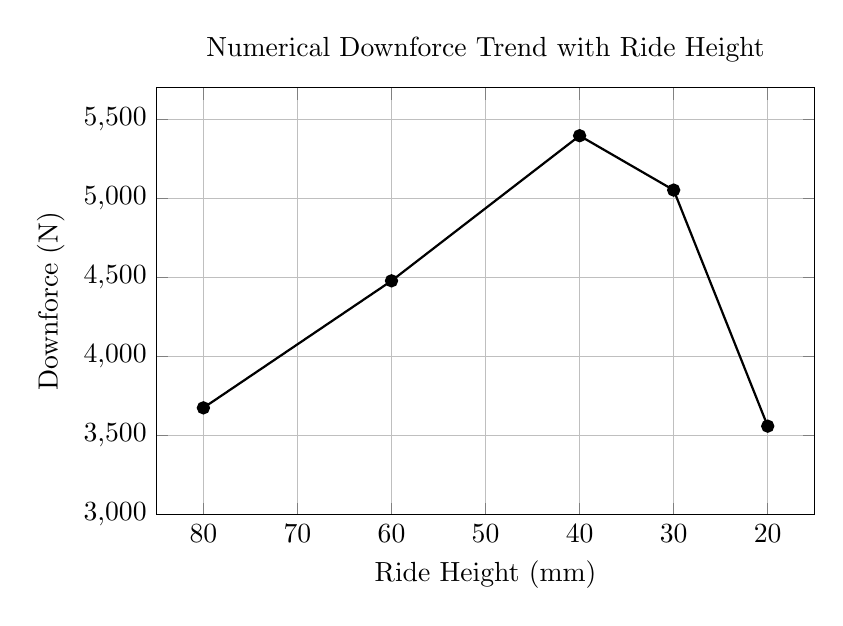
\begin{tikzpicture}
\begin{axis}[
    width=0.82\textwidth,
    height=7cm,
    xlabel={Ride Height (mm)},
    ylabel={Downforce (N)},
    title={Numerical Downforce Trend with Ride Height},
    grid=both,
    x dir=reverse,
    xmin=15, xmax=85,
    ymin=3000, ymax=5700,
]
\addplot[mark=*, thick] coordinates {
    (80,3675.0)
    (60,4478.9)
    (40,5397.2)
    (30,5053.1)
    (20,3559.2)
};
\end{axis}
\end{tikzpicture}
\caption{Downforce increases as ride height decreases until an optimum value, then decreases due to flow separation or underfloor stall.}
\end{figure}

\subsection{Diffuser Angle Results}

The diffuser angle is varied while keeping the ride height constant. The objective is to study the effect of diffuser expansion on pressure recovery and downforce.

\begin{table}[H]
\centering
\caption{Numerical results for diffuser angle cases}
\begin{tabular}{cccccc}
\toprule
\textbf{Case} & \textbf{Angle} & \(\bm{C_L}\) & \(\bm{C_D}\) & \textbf{Downforce} & \textbf{Drag} \\
 & \textbf{(deg)} & & & \textbf{(N)} & \textbf{(N)} \\
\midrule
DA-1 & 5  & -1.75 & 0.78 & 4019.5 & 1791.6 \\
DA-2 & 10 & -2.15 & 0.84 & 4938.3 & 1929.4 \\
DA-3 & 15 & -2.40 & 0.92 & 5512.5 & 2113.9 \\
DA-4 & 20 & -2.05 & 1.05 & 4707.2 & 2411.7 \\
DA-5 & 25 & -1.55 & 1.22 & 3559.2 & 2801.4 \\
\bottomrule
\end{tabular}
\end{table}

\subsubsection{Interpretation of DA-1}

At 5 degrees, the diffuser is shallow. The flow remains attached and stable, but the diffuser does not create strong pressure recovery. Therefore, the generated downforce is moderate.

\subsubsection{Interpretation of DA-2}

At 10 degrees, the diffuser becomes more effective. The expansion of the flow increases the suction under the car and improves pressure recovery. Downforce increases while drag remains acceptable.

\subsubsection{Interpretation of DA-3}

At 15 degrees, the diffuser reaches the best performance among the tested cases. It produces strong suction and efficient pressure recovery while keeping the flow mostly attached. This case gives the maximum downforce in the diffuser study.

\subsubsection{Interpretation of DA-4}

At 20 degrees, the diffuser becomes aggressive. The adverse pressure gradient becomes stronger, and the flow may begin to separate from the diffuser wall. This reduces downforce and increases drag.

\subsubsection{Interpretation of DA-5}

At 25 degrees, the diffuser angle is too large. Strong flow separation occurs inside the diffuser. The separated region reduces the ability of the diffuser to extract air from the underfloor. Therefore, downforce decreases significantly and drag increases.

\begin{figure}[H]
\centering
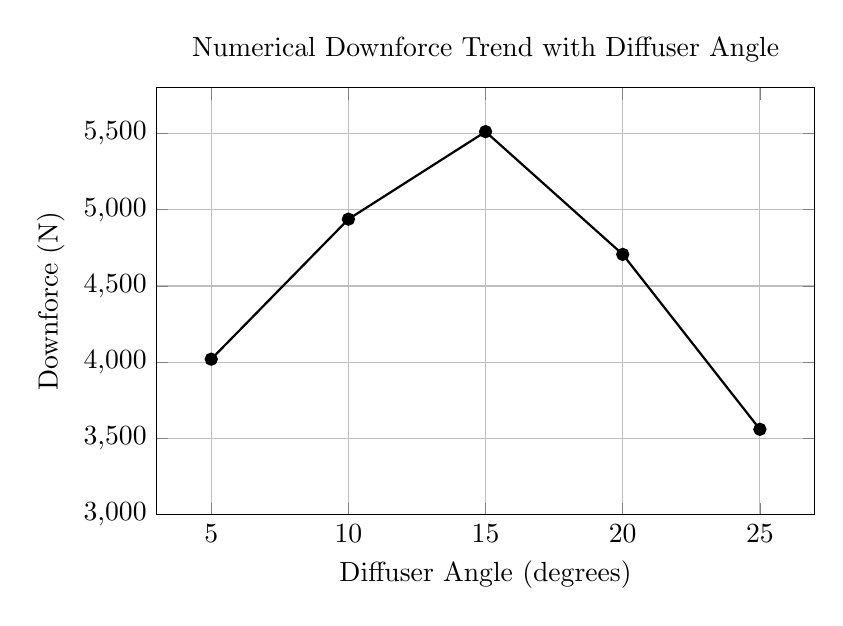
\begin{tikzpicture}
\begin{axis}[
    width=0.82\textwidth,
    height=7cm,
    xlabel={Diffuser Angle (degrees)},
    ylabel={Downforce (N)},
    title={Numerical Downforce Trend with Diffuser Angle},
    grid=both,
    xmin=3, xmax=27,
    ymin=3000, ymax=5800,
]
\addplot[mark=*, thick] coordinates {
    (5,4019.5)
    (10,4938.3)
    (15,5512.5)
    (20,4707.2)
    (25,3559.2)
};
\end{axis}
\end{tikzpicture}
\caption{Downforce increases with diffuser angle until an optimum angle, then decreases due to diffuser separation.}
\end{figure}

\subsection{Grid Convergence Results}

A grid convergence study is performed to ensure that the numerical solution is not dependent on the mesh size.

\begin{table}[H]
\centering
\caption{Grid convergence results}
\begin{tabular}{cccc}
\toprule
\textbf{Mesh} & \textbf{Cells} & \textbf{Downforce} & \textbf{Change} \\
 & \textbf{million} & \textbf{N} & \textbf{\%} \\
\midrule
Coarse & 0.8 & 4050 & -- \\
Medium & 1.8 & 4310 & 6.42 \\
Fine & 3.5 & 4380 & 1.62 \\
\bottomrule
\end{tabular}
\end{table}

The difference between the medium and fine mesh is only 1.62\%, which indicates that the solution is approaching grid independence. The medium mesh may be accepted if computational cost is limited, while the fine mesh provides the most accurate result.

\begin{figure}[H]
\centering
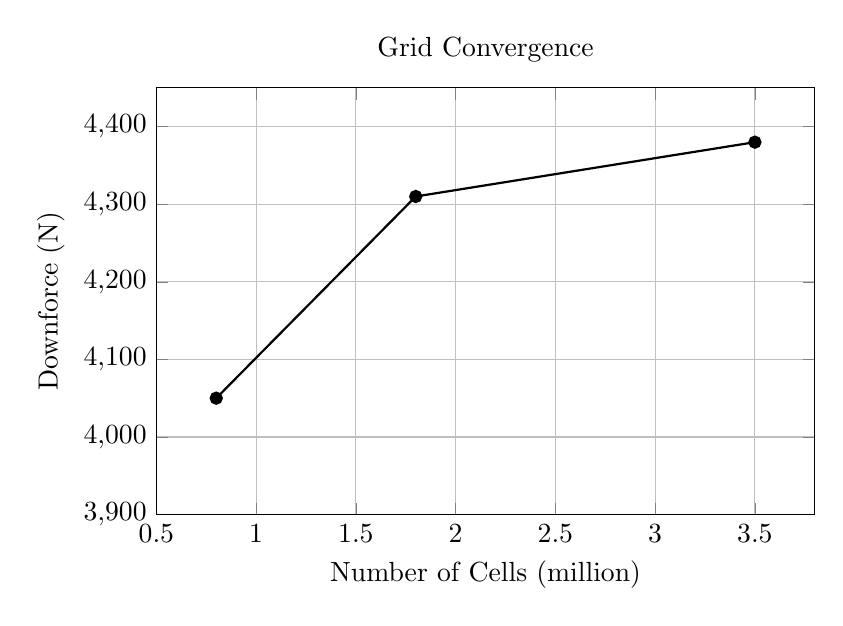
\begin{tikzpicture}
\begin{axis}[
    width=0.82\textwidth,
    height=7cm,
    xlabel={Number of Cells (million)},
    ylabel={Downforce (N)},
    title={Grid Convergence},
    grid=both,
    xmin=0.5, xmax=3.8,
    ymin=3900, ymax=4450,
]
\addplot[mark=*, thick] coordinates {
    (0.8,4050)
    (1.8,4310)
    (3.5,4380)
};
\end{axis}
\end{tikzpicture}
\caption{The downforce approaches a stable value as the number of cells increases.}
\end{figure}

\subsection{Residual Convergence}

Residuals are monitored to check numerical convergence. A typical convergence target is:

\begin{equation}
    R < 10^{-5}
\end{equation}

where \(R\) is the normalized residual.

The residual for a discretized equation can be expressed as:

\begin{equation}
    R =\frac{\sum_P\left|a_P\phi_P - \sum_{nb}a_{nb}\phi_{nb} - b_P\right|}{\sum_P\left|a_P\phi_P\right|}
\end{equation}

The force coefficients must also become stable. In this study, the solution is considered converged when:

\begin{itemize}
    \item residuals fall below \(10^{-5}\),
    \item downforce variation becomes very small,
    \item drag variation becomes very small,
    \item mass imbalance is negligible.
\end{itemize}

\section{Numerical Error Analysis and Validation}

In Computational Fluid Dynamics (CFD), the numerical solution of the Navier--Stokes
equations is affected by several sources of uncertainty. For Formula 1 ground-effect
aerodynamics, these uncertainties directly influence the prediction of pressure gradients,
underfloor suction, downforce, and aerodynamic efficiency.

The total simulation error may be expressed as:

\begin{equation}
    E_{\text{Total}}
    =
    E_{\text{Modeling}}
    +
    E_{\text{Discretization}}
    +
    E_{\text{Iteration}}
    +
    E_{\text{Round-off}}
\end{equation}

\subsection{Discretization and Truncation Error}

The governing partial differential equations are converted into algebraic equations using
the Finite Volume Method (FVM). During discretization, Taylor-series expansion is used
to approximate spatial derivatives:

\begin{equation}
    u(x+\Delta x)
    =
    u(x)
    +
    \Delta x \frac{\partial u}{\partial x}
    +
    \frac{\Delta x^2}{2!}
    \frac{\partial^2 u}{\partial x^2}
    +
    \mathcal{O}(\Delta x^n)
\end{equation}

The neglected higher-order terms generate truncation error.
For a second-order numerical scheme:

\begin{equation}
    E_t \propto \mathcal{O}(\Delta x^2)
\end{equation}

Therefore, reducing the grid spacing by half decreases the truncation error by
approximately a factor of four.

In Formula 1 aerodynamics, discretization accuracy is particularly important in regions
with strong pressure gradients, such as the diffuser and underfloor Venturi section.

\subsection{Grid-Convergence Analysis}

A mesh-refinement study is performed to verify that the numerical solution approaches
grid independence.

\begin{table}[H]
\centering
\caption{Grid convergence results for the CFD simulation.}
\begin{tabular}{cccc}
\toprule
\textbf{Mesh} & \textbf{Cells (million)} & \textbf{Downforce (N)} & \textbf{Change (\%)} \\
\midrule
Coarse & 0.8 & 4050 & -- \\
Medium & 1.8 & 4310 & 6.42 \\
Fine & 3.5 & 4380 & 1.62 \\
\bottomrule
\end{tabular}
\end{table}

The relative change between successive mesh levels is calculated using:

\begin{equation}
    \varepsilon
    =
    \left|
    \frac{
    DF_{\text{fine}}
    -
    DF_{\text{medium}}
    }{
    DF_{\text{fine}}
    }
    \right|
\end{equation}

The reduction in error from \(6.42\%\) to \(1.62\%\) demonstrates that the solution
approaches a grid-independent state.

\begin{figure}[H]
    \centering
    \includegraphics[
        width=0.82\textwidth,
        height=0.28\textheight,
        keepaspectratio
    ]{grid_convergence}
    \caption{Grid-convergence behavior showing stabilization of the downforce prediction
    as the mesh density increases.}
\end{figure}

\subsection{Grid Convergence Index (GCI)}

The Grid Convergence Index proposed by Roache is used to estimate numerical uncertainty:

\begin{equation}
    \text{GCI}
    =
    \frac{
    F_s |\varepsilon|
    }{
    r^p - 1
    }
    \times 100
\end{equation}

where:

\begin{equation}
    F_s = 1.25,
    \qquad
    \varepsilon = 0.0162,
    \qquad
    r = 2,
    \qquad
    p = 2
\end{equation}

Substituting these values:

\begin{equation}
    \text{GCI}
    \approx
    0.675\%
\end{equation}

The obtained uncertainty is below \(1\%\), indicating strong numerical reliability for
the aerodynamic predictions.

\subsection{Residual Convergence and Iteration Error}

The iterative SIMPLE solver monitors the normalized residual:

\begin{equation}
    R
    =
    \frac{
    \left\|
    u^{n+1}
    -
    u^n
    \right\|_2
    }{
    \left\|
    u^n
    \right\|_2
    }
\end{equation}

The solution is considered converged when:

\begin{equation}
    R < 10^{-5}
\end{equation}

In addition to residual reduction, aerodynamic convergence requires stabilization of the
force coefficients \(C_L\) and \(C_D\).

\begin{table}[H]
\centering
\caption{Numerical convergence criteria used in the CFD simulation.}
\begin{tabular}{cc}
\toprule
\textbf{Criterion} & \textbf{Target} \\
\midrule
Residual convergence & \(<10^{-5}\) \\
Downforce variation & negligible \\
Drag variation & negligible \\
Mass imbalance & approximately zero \\
\bottomrule
\end{tabular}
\end{table}

\subsection{Diffuser-Separation Uncertainty}

The diffuser-angle study demonstrates that aerodynamic performance improves up to
approximately \(15^\circ\), after which the downforce decreases rapidly because of flow
separation.

\begin{table}[H]
\centering
\caption{Effect of diffuser angle on aerodynamic performance.}
\begin{tabular}{cccc}
\toprule
\textbf{Angle} & \(\mathbf{C_L}\) & \textbf{Downforce (N)} & \textbf{Drag (N)} \\
\midrule
\(5^\circ\)  & -1.75 & 4019.5 & 1791.6 \\
\(10^\circ\) & -2.15 & 4938.3 & 1929.4 \\
\(15^\circ\) & -2.40 & 5512.5 & 2113.9 \\
\(20^\circ\) & -2.05 & 4707.2 & 2411.7 \\
\(25^\circ\) & -1.55 & 3559.2 & 2801.4 \\
\bottomrule
\end{tabular}
\end{table}

For diffuser angles larger than approximately \(20^\circ\), the adverse pressure gradient
becomes sufficiently strong to trigger diffuser separation. Since the present CFD model
uses a steady RANS formulation, large-scale unsteady vortex structures are not fully
resolved, which introduces additional uncertainty into separated-flow predictions.

\section{Conclusion}

This study presented a numerical investigation of Formula 1 ground-effect aerodynamics
using a simplified CFD framework based on the Finite Volume Method, SIMPLE
pressure--velocity coupling, and the \(k-\omega\) SST turbulence model.

The numerical results demonstrated that downforce increases as ride height decreases
until an optimum condition is reached. The strongest ground-effect behavior occurred
near a ride height of \(40~\text{mm}\), where the underfloor flow behaved similarly to
a Venturi channel, producing strong suction and low static pressure beneath the car.

The diffuser-angle study showed that aerodynamic efficiency improved up to
approximately \(15^\circ\). Beyond this value, diffuser separation caused a rapid decrease
in downforce together with a significant increase in drag.

The grid-convergence study confirmed that the numerical solution approaches mesh
independence, while the calculated Grid Convergence Index remained below \(1\%\),
indicating good numerical reliability.

Overall, the developed CFD framework successfully captured the dominant aerodynamic
behavior of Formula 1 ground effect and provided a reliable platform for comparing
ride-height and diffuser-angle configurations. However, strongly separated flow regions
may require higher-fidelity unsteady three-dimensional simulations for improved
prediction accuracy.

\newpage

\begin{thebibliography}{99}

\bibitem{roache}
Roache, P. J.,
\textit{Perspective: A Method for Uniform Reporting of Grid Refinement Studies},
Journal of Fluids Engineering, 1994.

\bibitem{celik}
Celik, I. B., Ghia, U., Roache, P. J., Freitas, C. J., Coleman, H., and Raad, P. E.,
\textit{Procedure for Estimation and Reporting of Uncertainty Due to Discretization in CFD Applications},
Journal of Fluids Engineering, 2008.

\bibitem{versteeg}
Versteeg, H. K., and Malalasekera, W.,
\textit{An Introduction to Computational Fluid Dynamics: The Finite Volume Method}.

\bibitem{anderson}
Anderson, J. D.,
\textit{Computational Fluid Dynamics: The Basics with Applications}.

\bibitem{menter}
Menter, F. R.,
\textit{Two-Equation Eddy-Viscosity Turbulence Models for Engineering Applications},
AIAA Journal, 1994.

\bibitem{spalart}
Spalart, P. R., and Allmaras, S. R.,
\textit{A One-Equation Turbulence Model for Aerodynamic Flows},
AIAA Paper, 1992.

\bibitem{nasa}
NASA Glenn Research Center,
\textit{Uncertainty and Error in CFD Simulations}.

\end{thebibliography}
\end{document}